\documentclass[a4paper,12pt]{book}

\usepackage[T1]{fontenc}	% Codifica di output
\usepackage[utf8]{inputenc}	% Codifica di input
\usepackage[italian]{babel}	% Lingua del documento

\usepackage{graphicx}
\usepackage{wrapfig}

\usepackage{float} % entativo di fissaggio immagini

\usepackage[table,xcdraw]{xcolor}
\definecolor{light-gray}{gray}{0.95}
\usepackage{enumitem}
\usepackage{amsmath,amssymb,amsthm}	% Pacchetti per la matematica
\usepackage{units}


\begin{document}

\author{Bozzo Francesco \and Conti Samuele \and Daniotti Filippo}
\title{Appunti Calcolatori Elettronici}
\date{Febbraio 2019}

\frontmatter
\maketitle
\tableofcontents

\mainmatter
\chapter{Introduzione ai calcolatori}

\section{Un po' di storia dell'informatica}
\paragraph{ENIAC, il primo computer della storia}
Commissionato nel 1946 dal Dipartimento di Difesa degli Stati Uniti, \textbf{ENIAC} (\textit{Electonic Numerical Integrator and Computer}) diventa il primo calcolatore della storia.
Dotato di $18000$ valvole termoioniche, esso occupava una stanza di 9x30 metri, consumando un ammontare spropositato di energia.\\
Il suo impiego principale consisteva nel calcolare traiettorie dei proiettili di artiglieria. Infatti, è doveroso specificare come i primi calcolatori della storia siano stati concepiti per essere sfruttati in applicazioni belliche.

\paragraph{Apollo Guidance Computer}
Prodotto da IBM nel 1969, disponeva di 2800 circuiti integrati, un processore da \unit[0.043]{MHz} e \unit[152]{KByte}  complessivi di memoria ROM/RAM. Presentava un'interfaccia display\&keyboard: i comandi utilizzano una sintassi del tipo "verbo + nome".

\paragraph{Programma 101} Nel 1964 l'Olivetti rilascia il primo \textit{personal computer} della storia, sfortunatamente non avrà successo. 

\subsection{Differenziazione dei calcolatori}
Seppur i calcolatori di oggi condividano la stessa idea base, le soluzioni per ciascuna tipologia di applicazione sono piuttosto diverse. A seguire alcuni esempi di diverso tipo di calcolatori:
\begin{table}[h!]
	\begin{tabular}{|l|l|l|l|}
		\hline
		\rowcolor[HTML]{EFEFEF} 
		Tipologia di calcolatore & Costo   & Prestazioni                     & Applicazioni                     \\ \hline
		&         &                                 & Software prodotti da             \\
		Personale                & Ridotto & \multicolumn{1}{c|}{Buone}      & terze parti                      \\
		&         &                                 &                                  \\ \hline
		&         &                                 & Poche ma complesse (calcolo      \\
		Server                   & Elevato & \multicolumn{1}{c|}{Eccellenti} & scientifico) o tante ma semplici \\
		&         &                                 & (web server)                     \\ \hline
		&         & \multicolumn{1}{c|}{Minime}     & Dedicate e molto specifiche;     \\
		Embedded                 & Minimo  & \multicolumn{1}{c|}{necessarie} & esiste un vasto spettro di scopi \\
		&         &                                 & possibili                        \\ \hline
	\end{tabular}
\end{table}
Per ovvi motivi, ogni tipologia di calcolatore è meglio adatta per differenti scopi. Ottenere delle buone prestazioni senza eccedere in prezzo e potenza è ciò che decreta il successo commerciale di un prodotto.

\section{Le prestazioni dei calcolatori}
Un buon programmatore, oltre a saper utilizzare degli efficienti paradgmi, deve comprendere la gerarchia di memoria e il concetto di parallelismo: conoscere a fondo il calcolatore è fondamentale.\\
Fino a qualche tempo fa le prestazioni di qualsiasi calcolatore erano in balia della disponibilità di memoria. Al giorno d'oggi invece risulta un problema risolto, tranne per qualche criticità per le applicazioni embedded.\\
Ecco una lista degli elementi che influenzano le prestazioni del calcolatore e il loro ruolo:
\begin{itemize}[noitemsep, nolistsep]
	\item \textit{Algoritmi}: determinano il numero di istruzioni di alto livello e di operazioni di IO.
	\item \textit{Linguaggi di programmazione, compilatori e architetture}: determinano il numero di istruzioni macchina per ogni istruzione di basso livello.
	\item \textit{Processore e sistema di memoria}: determina quanto velocemente è possibile eseguire ciascuna istruzione.
	\item \textit{Sistema di I/O (Hardware e sistema operativo)}: determina quanto velocemente possono essere eseguite le istruzioni.
\end{itemize}

\subsection{La memoria e il processore}
\paragraph*{La memoria}
\`{E} possibile classificare la memoria in:
\begin{itemize}[noitemsep]
	\item \textit{volatile}: è costituita da vari banchi di (tipicamente) 8 chip di RAM dinamica. \`{E} dominata dalle \textit{DRAM}.
	\item \textit{permanente}: è costituita da memorie flash (es. SSD), dischi rigidi e CD/DVD.
\end{itemize}
La prima viene utilizzata per memorizzare dati e programmi mentre vengono eseguiti (per questo motivo viene chiamata anche \textit{memoria principale}): allo spegnimento i dati vengono persi. La seconda viene usata per memorizzare grandi quantità di dati e programmi fra esecuzioni diverse.\\
Il principio di funzionamento dell'hard disk è di magnetizzare delle particelle metalliche distribuite su un substrato:
\begin{itemize}[noitemsep]
	\item I dischi sono organizzati in strutture sovrapposte (cilindri).
	\item Le particelle vengono lette da un dispositivo meccanico (testina) che si sposta radialmente su un braccio (in grado di fare movimenti angolari).
	\item Questa componente rallenta i tempi di accesso ma aumenta al densità di memorizzazione (è possibile arrivare facilmente ai Terabyte).
\end{itemize}

Diversamente dai dischi rigidi elettromeccanici, la memorizzazione su una memoria flash avviene intrappolando una carica elettrica in maniera permanente.\\
I dischi ottici funzionano sul principio di riflessione della luce: viene emesso un raggio laser che viene riflesso dai rilievi, nel caso bit 1, e assorbito dalle buche, nel caso bit 0. Nei dischi riscrivibili è inoltre presente un particolare substrato che se riscaldato torna alla condizione di partenza, eliminando tutti i dati memorizzati.

\paragraph*{Il processore}
La \textbf{CPU} è l'unità centrale di ogni calcolatore. Si compone di:
\begin{itemize}[noitemsep]
	\item \textit{Datapath}: esegue operazioni aritmetiche sui dati.
	\item \textit{Control Unit}: impartisce ordini al datapath, alla memoria e alle componenti IO, sulla base di quanto stabilito dal programma.
\end{itemize}
Il processore offre l'\textbf{ISA} (\textit{Instruction Set Architecture}), un'interfaccia che permette di utilizzarlo senza conoscerne i dettagli. In aggiunta all'ulteriore interfaccia del sistema operativo, insieme formano l'interfaccia binaria delle applicazioni \textbf{ABI} (\textit{Application Binary Interface}). Ciò permette allo sviluppatore di svincolarsi dal livello hardware sottostante, secondo il principio di \textit{astrazione}.\\ Esistono due diversi tipi di architetture ISA:
\begin{itemize}[noitemsep,nolistsep]
	\item \textbf{RISC}: offre un numero ridotto di istruzioni, rivolta soprattutto a sistemi \textit{embedded};
	\item \textbf{CISC}: offre Permette di usufruire di un maggior numero di istruzioni, rivolta prevalentemente ai PC.
\end{itemize}

\subsection{Software di sistema}
Il \textit{sistema operativo}:
\begin{itemize}[noitemsep]
	\item gestisce le operazioni di I/O.
	\item alloca la memoria.
	\item consente il multitasking.
\end{itemize}
Il \textit{compilatore} traduce da linguaggio ad alto livello a linguaggio macchina. Ogni istruzione di quest'ultimo è costituita da una determinata sequenza di \textit{bit}, ossia l'unità di base dell'informazione (1 o 0).\\
L'utilità del compilatore consiste nel facilitare il lavoro del programmatore: non è più necessario implementare il software in codice binario, bensì è possibile utilizzare un linguaggio di programmazione più vicino al linguaggio naturale. Il primo linguaggio sviluppato per questo scopo è stato l'\textit{assembly}. Il software che traduce l'assembly in codice binario si chiama \textit{assembler}.\\
\`{E} possibile riassumere la traduzione di un linguaggio di programmazione di alto livello in codice macchina in due semplici passi:
\begin{enumerate}[noitemsep]
	\item traduzione del linguaggio ad alto livello in linguaggio assembly, per via del compilatore
	\item traduzione del linguaggio assembly in linguaggio macchina, attraverso l'assemblatore.
\end{enumerate}
Spesso fanno eccezione alcuni compilatori che trasformano direttamente il linguaggio ad alto livello in codice macchina.

\subsection{Periferiche di IO}
Il \textbf{mouse} è stato inventato nel 1967 da \textit{Doug Engelbart} nei laboratori della \textit{Xerox}. Attualmente sfrutta la tecnologia ottica: attraverso le variazioni di luce provocate da alcuni led che illuminano il piano, il mouse è in grado di rilevare gli spostamenti.

Gli schermi \textbf{LCD} (\textit{Liquid Crystal Display}) sono costituiti da alcuni cristalli che galleggiano in un fluido: ciascuno di essi corrisponde ad un pixel. Attraverso un campo elettrico è possibile ruotare di 90 gradi ogni singolo cristallo, che di conseguenza può impedire o meno il passaggio della luce secondo il fenomeno fisico della \textit{luce polarizzata}.\\
L'immagine dunque viene rappresentata da una matrice di pixel: ciascuno di essi ha associata una componente rosso, verde, blu (sistema RGB). Questa immagine viene memorizzata in un \textit{frame buffer}, una RAM che viene aggiornata  fino a 100 volte al secondo.

\subsection{Misurazione delle prestazioni}
I moderni processori sono costruiti usando un segnale periodico che ne sincronizza le operazioni. Il \textit{ciclo di clock} è l’intervallo di tempo che intercorre tra due colpi di clock. La frequenza è definita come $\frac{1}{\text{ciclo clock}}$. Il ciclo di clock è misurato in secondi, la frequenza in Hertz.\\

Il tempo necessario per l'esecuzione di un programma dipende da tre fattori:
\begin{itemize}[nolistsep]
	\item il numero di istruzioni dell'algoritmo.
	\item i cicli di clock per istruzione (\textit{CPI}).
	\item la frequenza di clock.
\end{itemize}
\begin{equation*}
\text{Tempo CPU} = \text{Num Istruzioni } \cdot \text{ CPI } \cdot \text{ Periodo Clock} = \frac{\text{Num Istruzioni} \cdot \text{CPI}}{\text{Frequenza Clock}}
\end{equation*}

\begin{figure}[H]
	\centering
	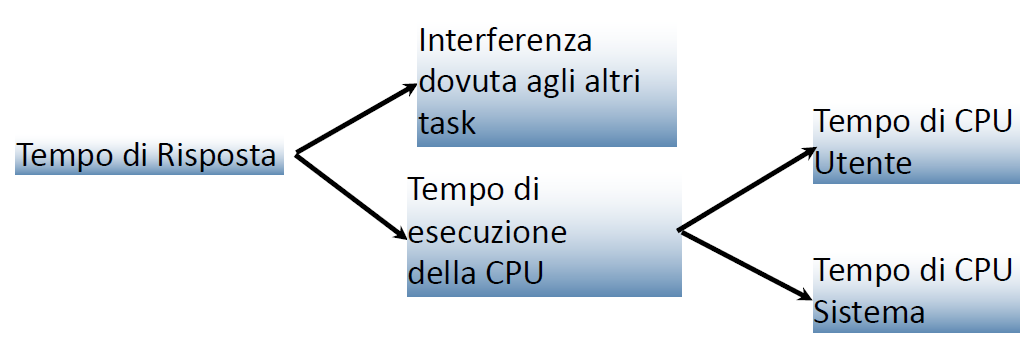
\includegraphics[width=0.9\textwidth,keepaspectratio]{images/tempo_risposta.png}
	\caption{Diagramma del tempo di risposta}
\end{figure}
Un algoritmo è efficiente se viene strutturato in modo da risparmiare istruzioni e, per una particolare architettura, se utilizza le istruzioni più efficienti (quelle con un basso CPI, poichè il CPI dei diversi tipi di istruzione varia in base all'architettura che deve svolgere le istruzioni).\\
Il linguaggio di programmazione influenza il numero di istruzioni e il CPI: più di alto livello sono i costrutti, più lunghe sono le sequenze di istruzioni macchina ottenute traducendo il codice di partenza.\\
Il compilatore sicuramente influenza sia il numero di istruzioni che il CPI in base alla propria efficienza e ottimizzazione.\\
Anche l'\textit{ISA} ha impatto sul numero di istruzioni, sul CPI, e sulla frequenza di clock attraverso la sua progettazione: essa può fornire istruzioni di basso o alto livello (più o meno istruzioni per eseguire un'operazione).

\subsection{La legge di Moore}
Negli scorsi anni le prestazioni dei calcolatori sono aumentati costantemente, secondo l'andamento previsto da \textit{Moore} attraverso una legge informale.\\
Di recente si è assistito a una diminuzione dell’incremento tra una generazione e l’altra, sintomo di una evidente saturazione, casuata da limiti fisici della materia.

\subsection{La barriera dell'energia}
Dagli anni Ottanta ad oggi, la frequenza media dei processori è stata aumentata di più di mille volte, con conseguente aumento dei consumi di 30 volte.
\begin{equation*}
\text{Potenza} = \text{capacità}\cdot \text{tensione}^2\cdot \text{frequenza di commutazione}
\end{equation*}
Dove la frequenza di commutazione è legata alla frequenza di clock.\\
Incrementare la frequenza senza eccedere in consumi è stato permesso grazie un abbassamento della tensione di alimentazione (termine quadratico, quindi il più influente) da \unit[5]{V} a \unit[1.2]{V}. Al di sotto di questo valore avvengono fenomeni di tipo elettrostatico che portano il sistema in una condizione anomala.\\
C’è inoltre un limite alla capacità di estrarre la potenza prodotta dai processori (e il conseguente calore) tramite ventole o radiatori. Il processo di refrigerazione diventa molto
costoso e difficilmente attuabile in dispositivi desktop e laptop.\\

La soluzione principale che è stata adottata consiste nelle \textit{architetture multicore} sfruttando il concetto di \textit{parallelismo}. Ciò comporta una maggiore difficoltà e responsabilità nella scrittura di codice da parte del programmatore (debugging complicato, bilanciare il carico di lavoro fra le CPU).





\documentclass[class=book, crop=false]{standalone}
\usepackage[subpreambles=true]{standalone}

\usepackage{../../style}

\graphicspath{{./assets/images/}}

\begin{document}
\chapter{Aritmetica dei calcolatori}
\section{Informazione nei computer}

\subsection{I transistor}
\begin{wrapfigure}{r}{0.4\textwidth}
	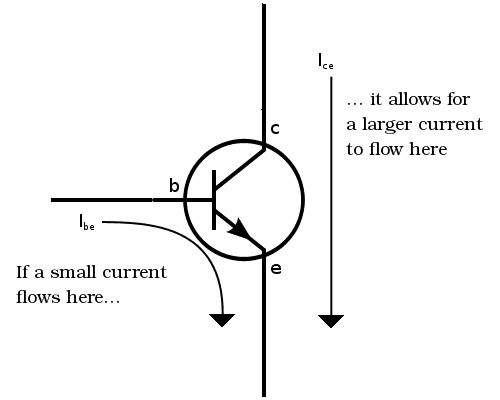
\includegraphics[width=0.9\linewidth]{transistor.png}
	\label{fig:transistor}
	\centering
\end{wrapfigure}
Tutti i computer moderni sono composti da \emph{transistor} (detti anche triodi), delle strutture bistabili: possono assumere due stati come un interruttore, 0 (spento) e 1 (acceso). Molti \emph{transistor} collegati tra loro in una sorta di matrice possono rappresentare delle serie di porte logiche, ed è questa la struttura che sta alla base dell'architettura dei moderni calcolatori.\\
Un computer memorizza (e manipola) solo sequenze di 0 e 1 (sequenze di bit); anche l’ENIAC funzionava allo stesso modo, solo che al posto dei \emph{transistor} era composto da \emph{valvole termoioniche}, che non erano differenti nel funzionamento (assumono sempre i due stati descritti in precedenza, solo più lentamente).
\subsection{Interpretazione delle informazioni} In seguito le sequenze di bit che i computer elaborano/memorizzano possono essere interpretate in tantissimi modi diversi, tra cui numeri, caratteri, suoni, immagini, istruzioni e molti altri.\\
Alla base di tutte le interpretazioni che si possono dare alle stringhe di simboli (che nel caso del computer sono proprio i due stati del bit) sta il concetto di codifica. La \emph{codifica} è appunto uno schema, una legge, un \emph{mapping} che permette prima di tradurre, poi di interpretare stringhe di simboli.
Nell’ambito dell’IT le codifiche sono fortemente caratterizzate dalla lunghezza (dal numero di bit) delle “parole” elementari della codifica. Ad esempio, per rappresentare tutti i caratteri (tabella ASCII) utilizziamo  8 bit [256 caratteri].
Si osservi che essendo i \emph{transistor} sistemi bistabili la base 2 (con cifre 0 e 1) è perfetta per rappresentare la codifica dei dati memorizzati/elaborati da essi.
\section{I numeri}
Limitiamoci al caso dei numeri per spiegare il concetto di \emph{codifica}:\\
Ricordiamo che i  metodi di rappresentazione numerica che studiamo sono posizionali, ovvero il peso di ogni cifra varia in base alla posizione che essa  occupa.\\
In generale se una base è composta da B elementi essa ha B cifre (da 0 a B-1) utilizzate per scrivere ogni numero.
Questa formula ci restituisce il valore di ogni numero scritto in una qualsiasi base B:\\
\[c_{i} c_{i-1} c_{i-2}... c_{0}=c_{i}\cdot B^{i}+...+c_{0}\cdot B^{0}\]\\
dove $c_{i}$ è la cifra in posizione \emph{i}.

\subsection{Regole di conversione tra basi}
Vediamo ora come operare la conversione tra le principali basi:
\begin{itemize}[noitemsep,nolistsep]
	\item \emph{da base 2 a base 16}: partendo da destra, si dividano le cifre binarie in gruppi da 4 cifre ciascuno, e ognuno di questi corrisponderà a una cifra esadecimale; qualora il numero di cifre binarie non sia divisibile per 4, si completi con degli 0 in modo da ottenere gruppi da 4\\ (\emph{esempio: $(11011)_{2}$ diventerà $(0001\text{ }1011)_{2}$, ovvero $(1B)_{16}$});
	\item \emph{da base 2 a base 8}: analogamente, si dividano le cifre binarie in gruppi da 3 cifre ciascuno, e ognuno di questi corrisponderà a una cifra ottale;
	\item \emph{da una qualsiasi base $B$ a base 10}: come visto sopra, si moltiplichi ogni cifra $c_{i}$ per $B^{i}$, dipendentemente dalla sua posizione;
	\item \emph{da base 10 a una qualsiasi base B}:
	\begin{enumerate}[noitemsep,nolistsep]
		\item si consideri un numero $x_{10}$ e una base $B$;
		\item si divida $x$ per $B$;
		\item il resto della divisione è la cifra da inserire a sinistra nel numero convertito;
		\item si assegni a $x$ il quoziente della divisione;
		\item si torni al punto 2 e si ripeta finché $x\neq0$.
	\end{enumerate}
\end{itemize}
\begin{figure}[H]
	\centering
	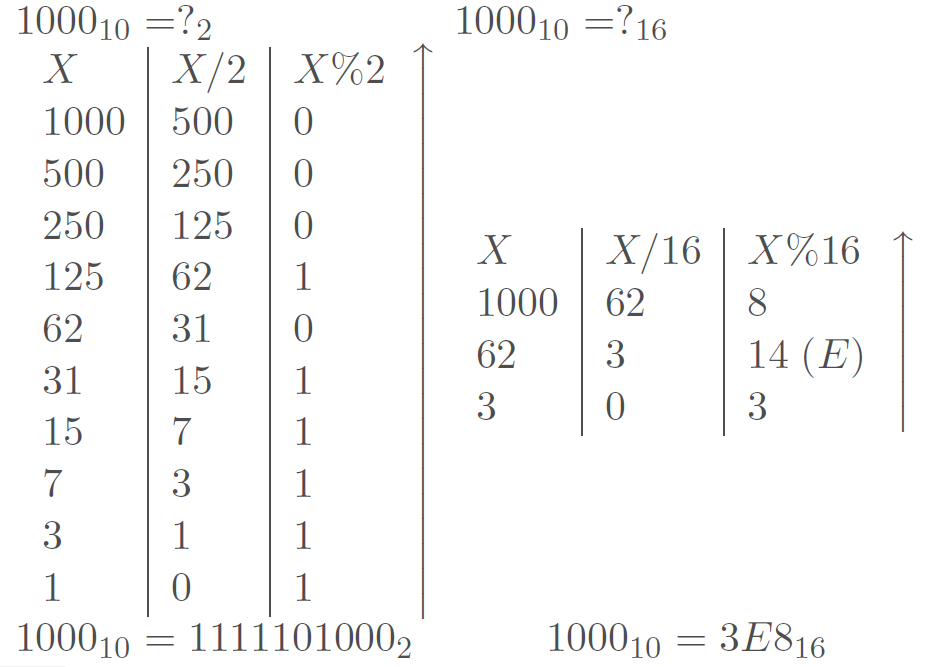
\includegraphics[width=0.7\textwidth,keepaspectratio]{esempi_conversioni.png}
	\caption{Alcuni esempi di conversione}
\end{figure}

\subsection{I naturali} Nella codifica binaria un numero naturale è rappresentato su \emph{k} cifre binarie, dove con \emph{k} cifre si possono rappresentare i numeri tra 0 e $2^{k}-1$.\\
La codifica più comune per gli interi spesso usa i byte, sequenze di 8 bit, che tuttavia richiedono molte cifre per rappresentare un numero e quindi spesso, per semplificare la lettura, si usa scrivere i numeri in esadecimale (quindi scrivendo un quarto delle cifre rispetto alla binaria).

\paragraph*{Somma e sottrazione}
Le operazioni somma e sottrazione funzionano allo stesso modo del sistema utilizzato nella numerazione decimale con il riporto. Si guardino gli esempi qui sotto riportati, già di per sè esplicativi del processo:\\

\begin{table}[H]
	\centering
	\subimport{assets/tables/}{es_somma.tex}
	\caption{Esempio di somma}
\end{table}

\begin{table}[H]
	\centering
	\subimport{assets/tables/}{es_diff.tex}
	\caption{Esempio di differenza}
\end{table}

\paragraph*{Moltiplicazione} La moltiplicazione in base binaria si può semplificare con il metodo dello shifting, che è più facile illustrare con un esempio:
\begin{table}[H]
	\centering
	\subimport{assets/tables/}{es_prod.tex}
	\caption{Esempio di prodotto}
\end{table}
Si noti che quando è presente un 1 si riscrive il numero (nella posizione corrispondente) mentre  quando è presente uno 0 semplicemente non si scrive nulla (e si va solo avanti con le posizioni).

\subsection{Gli interi} Finora abbiamo visto come si codificano solo i numeri naturali, ma esistono metodi di codifica che permettono di rappresentare anche i numeri negativi (quindi l’insieme degli interi). Le tecniche più comuni sono: modulo e segno, complemento a 1 (\emph{CA1}) e complemento a 2 (\emph{CA2}).

\paragraph*{Codifica con Modulo e Segno:} Idea semplice: si usano $k-1$ bit per rappresentare il valore assoluto (modulo) del numero  ed un bit per codificare il segno (0 per i positivi, 1 per i negativi). In questo modo con k bit si possono codificare valori tra $-2^{k-1}+1 \text{ e} +2^{k-1}-1$.\\
\emph{N.B.}: esistono due codifiche per lo $0$, $-0$  e $+0$, e questo è un spreco.

\paragraph*{Codifica in Complemento a 1:} L’idea alla base è semplice: il primo bit indica sempre il segno e per ottenere l’opposto di un numero positivo si invertono tutti gli 0 in 1 e gli 1 in 0 (e lo stesso si fa per ottenere l’opposto di un numero negativo). Si hanno ancora due rappresentazioni per +0 e -0 (rispettivamente, utilizzando 4 bit, 0000 e 1111). È più facile da sommare rispetto al modulo e segno ma solo se il bit significativo non dà riporto.
Quando si sommano due numeri in \emph{CA1}:
\begin{itemize}[noitemsep]
	\item si deve verificare che i riporti delle prime due cifre significative siano uguali, altrimenti il numero che si ottiene non è rappresentabile in CA1 su k bit.
	\item alla fine si deve sommare il riporto della prima cifra al risultato ottenuto (ultima riga).
\end{itemize}

\begin{figure}[H]
	\centering
	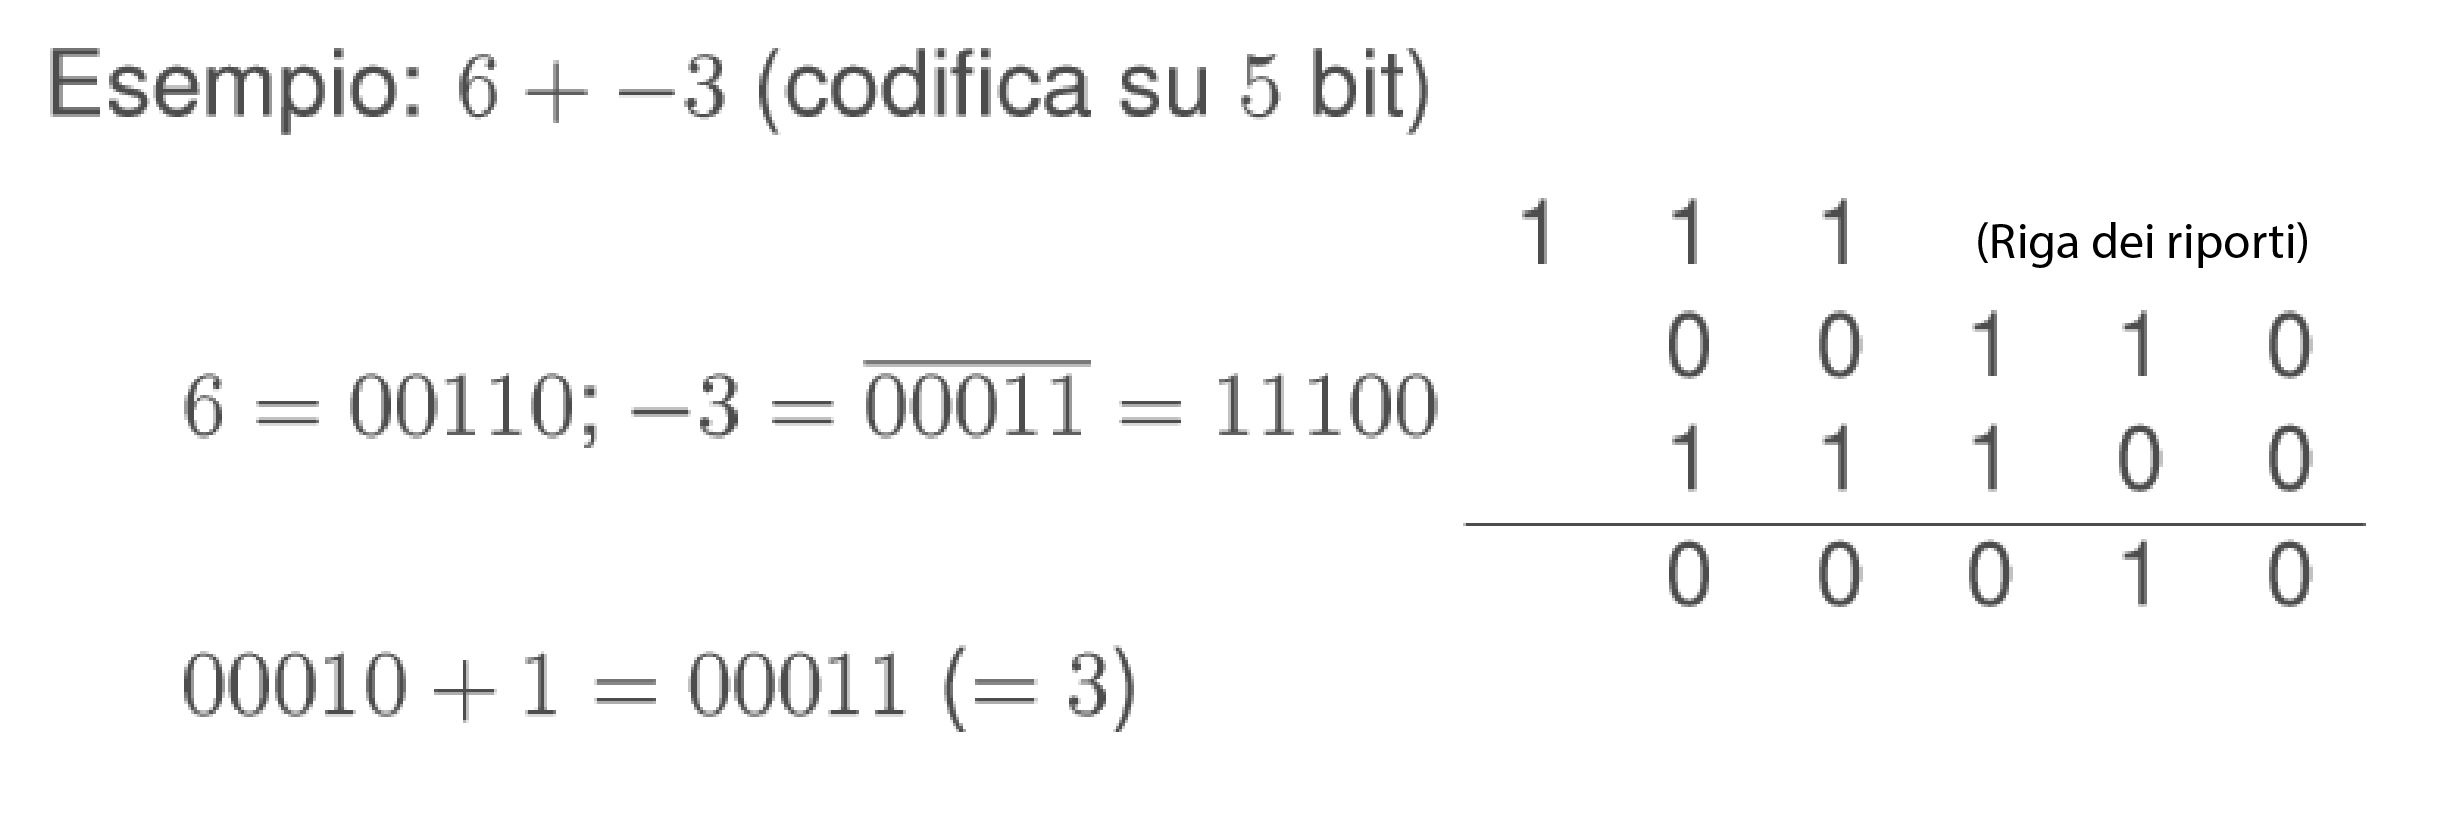
\includegraphics[width=0.9\textwidth,keepaspectratio]{Somma-CA1.png}
	\caption{Esempio di somma in CA1}
\end{figure}

\paragraph*{Codifica in Complemento a 2} Per tradurre un numero da intero con segno a complemento a 2 (\emph{CA2}) basta invertire tutti i bit e poi sommare 1. Viceversa, per convertire da \emph{CA2} a binario, si sottrae 1 e poi si invertono tutti i bit. \\
Ancora una volta il bit più significativo indica il segno, ma in questo caso la codifica dello 0 è unica, quindi con \emph{k} bit si possono rappresentare i numeri da $-2^{k-1}$ a $2^{k-1}-1$. Anche la somma è più semplice ma questo lo vedremo in futuro.

\subsubsection{Somma algebrica in Complemento a 2} L'utilizzo della codifica \emph{CA2} permette di eseguire somme algebriche senza alcuna differenza operativa, ma rende necessario prestare attenzione agli \emph{overflow}.\\
Con il termine \emph{overflow} si intende la situazione in cui, date in input delle informazioni codificate in un numero $k$ di bit arbitrariamente scelto, lo stesso numero $k$ di bit non è sufficiente a codificare le informazioni in output. \\
Diamo subito un esempio: supponiamo di voler eseguire $-64-8$ utilizzando il \emph{CA2} e $k=7$ bit. Ricordiamo che:\\\\
$-64=1000000_{2}=\overline{1000000}+1=0111111+1=1000000 \text{ in \emph{CA2;}}$\\
$-8=0001000_{2}=\overline{0001000}+1=1110111+1=1111000 \text{ in \emph{CA2}}.$\\\\
A questo punto eseguiamo la somma algebrica:
\begin{table}[H]
	\centering
	\subimport{assets/tables/}{overflow_CA2.tex}
\end{table}
Si noti che il numero fra parentesi indica l'ultimo riporto, che chiaramente non possiamo inserire poiché sforerebbe i 7 bit.\\
Osserviamo così che, per $k=7$ bit, $-64-8=0111000_{2}=56_{10}$, che ovviamente non ci piace; concludiamo quindi che la somma algebrica $-64-8=-72$ \emph{non} è rappresentabile con soli $k=7$ bit.

Possiamo dire che, in generale, dati due numeri $a, b$ aventi lo stesso segno, avremo problemi di \emph{overflow} se
\begin{itemize}[noitemsep,nolistsep]
	\item $a+b>2^{k-1}-1$
	\item $a+b<-2^{k-1}$
\end{itemize}
ricordando che $-2^{k-1}\le a,b\le 2^{k-1}-1$.

\subsection{Aritmetica modulare} Incosapevolmente noi utilizziamo l'\emph{aritmetica modulare} quasi continuamente, nella nostra quotidianità; l'esempio più comune è quando sommiamo le ore, che sono organizzate in modulo 24 (da cui la denominazione ufficiosa di "Matematica dell'orologio"), ma anche minuti e secondi (modulo 60) e gli angoli (modulo 360).\\
Diamone una descrizione intuitiva: fissato un numero $n$ finito di valori, arrivato al numero più grande ($n-1$), al successivo avrò che $(n-1)+1=0$.\\
Per completezza, forniamo ora la relazione di equivalenza di due numeri in modulo $n$:
\begin{equation*}
\centering
a\equiv b \longleftrightarrow a\%n=b\%n
\end{equation*}

Quando noi eseguiamo delle operazioni sui numeri in base 2 su $k$ bit, stiamo lavorando in un ambiente in modulo $2^{k}$, e calcolando $a+b$ stiamo in realtà trovando $(a+b)\%2^{k}$, e i due valori saranno uguali se e solo se $a+b<2^{k}$, perché altrimenti ogni valore successivo ricomincerebbe da 0: questo è l'\emph{overflow}.\\
In particolare quando lavoriamo su numeri interi in \emph{CA2} dobbiamo ricordare che, se $-2^{k-1}\le a+b\le 2^{k-1}-1$ non avremo \emph{overflow}, altrimenti
\begin{itemize}[noitemsep,nolistsep]
	\item se $a+b<2^{k-1}-1$, otterremo $a+b+2^{k}$ $\longrightarrow$ \emph{overflow}
	\item se $a+b>-2^{k-1}$, otterremo $a+b-2^{k}$ $\longrightarrow$ \emph{overflow}
\end{itemize}

\subsection{I Reali} Non è sempre semplice codificare un numero reale $\alpha \in \mathbb{R}$, poiché di questo insieme fanno parte i numeri cosiddetti \emph{irrazionali}, che presentano infinite cifre non periodiche dopo la virgola (si pensi ad esempio a $\pi=3,14159...$, o $e=2.71828...$, o ancora $\sqrt{2}=1.41421...$).\\
Alcuni numeri non possono quindi essere rappresentati con un numero finito di bit, per cui ne rappresenteremo solo un'approssimazione, e per farlo abbiamo sviluppato due metodi: la rappresentazione a \emph{virgola fissa} (\emph{fixed point}) e quella a \emph{virgola mobile} (\emph{floating point}).

\subsubsection{Codifica in virgola fissa} Questo sistema di codifica prevede che, posto un numero $k$ di bit per la rappresentazione del numero, si impieghino $k-f$ bit per rappresentarne la parte intera, e i restanti $f$ bit per rappresentarne la parte razionale:
\begin{equation*}
\overbrace{\underbrace{c_{k-1}c_{k-2}\cdots c_{f}}_\text{$k-f$}\underbrace{\cdot c_{f-1}\cdots c_{0}}_\text{$f$}}^\text{$k$}
\end{equation*}
 Possiamo scrivere una formula generale più compatta. Supponiamo di voler convertire un numero $x_{10}$:
 \begin{equation*}
 x_{10}=\sum_{i=0}^{k-1} c_{i}B^{i-f}=\sum_{i=0}^{k-1} c_{i}B^{i}\cdot B^{-f}=(\sum_{i=0}^{k-1} c_{i}B^{i})\cdot B^{-f}
 \end{equation*}
 Detta in altri termini, convertiamo il numero da base 10 come se non avesse la virgola e poi moltiplichiamo per $B^{-f}$.\\
 Presentiamo vantaggi e svantaggi di questo tipo di codifica:
  \begin{itemize}[noitemsep,nolistsep]
  	\item le operazioni si possono svolgere senza alcuna differenza, se non l'accortezza di scalare il risultato;
  	\item il peso per la CPU è ridotto;
  	\item non ci sono errori di approssimazione, \emph{se il valore è rappresentabile};
  	\item iniziamo ad avere problemi quando lavoriamo con un ampio spettro di ordini di grandezza.
  \end{itemize}

\subsubsection{Codifica in virgola mobile}
Un qualsiasi numero reale può essere scritto anche nella forma $x=M\cdot B^{E}$ dove M si dice \emph{mantissa}, E \emph{esponente} e B è la base della rappresentazione (che nel nostro caso è la leggendaria base 2).\\
Questo metodo di rappresentazione, molto simile alla notazione scientifica standard, è implementato anche nell'informatica in più modi diversi ma alla base di tutti si riconosce lo stesso schema: \\
$x$ può essere rappresentato su \emph{k} bit utilizzando \emph{m} bit per il campo mantissa M ed $e=k-m$ bit per il campo esponente E; quest'ultimo permette in un certo senso di "spostare" la virgola; con esponenti negativi si avranno $x$ "piccoli" e viceversa con esponenti positivi si avranno $x$ "grandi".\\
Lo standard più comunemente utilizzato è l'IEEE 754 che, nei numeri \emph{float} a precisione singola (dove si usano 32 bit), ha questa struttura:
\begin{table}[h!]
	\centering
	\begin{tabular}{|l|l|l|}
		\hline
		\multicolumn{1}{|c|}{1 bit} & \multicolumn{1}{c|}{8 bit} & \multicolumn{1}{c|}{23 bit} \\ \hline
		Bit di segno                & Esponente                  & Mantissa                    \\ \hline
	\end{tabular}
\end{table}


Il bit di segno ha la funzione che già conosciamo, mentre il campo $E$ può contenere valori compresi tra 0 e 255% ($-2^{e-1}+1 < E \le 2^{e-1}-1$)
; questi ultimi due valori vengono utilizzati per funzioni speciali, mentre i valori da 1 a 254 compresi codificano l'esponente effettivo dei calcoli, che diremo $exp$\footnote{La notazione $exp$ è stata introdotta da noi autori della dispensa perchè ci è sembrata più chiara ed agile di quella utilizzata dal professore, chiediamo venia se questo genererà confusione}, in questo modo:
\begin{equation*}
exp=E-2^{e-1}-1
\end{equation*}
Nel nostro caso, $exp=E-127$. L'ultimo campo, la \emph{mantissa}, codifica un numero intero.
\paragraph{Come calcolare il valore di un \emph{float}} Il primo bit è utilizzato per indicare il segno, i successivi 8 per $E$ e i restanti 23 per la mantissa. La decodifica in decimale assume due forme in base al valore di $E$:
\begin{itemize}[noitemsep,nolistsep]
	\item se $E=0$, allora il numero in base 10 è $x_{10}=0.M \cdot 2^{0}$;
	\item se $E>0$, allora il numero in base 10 è $x_{10}=1.M \cdot 2^{exp}$, dove $exp$ è definito come qui sopra descritto.
\end{itemize}
Nel primo di questi due casi i numeri si dicono \emph{denormalizzati}, essi rappresentano tutti i numeri compresi tra 0 e 1; nel secondo caso i numeri si dicono \emph{normalizzati} [questa distinzione è stata aggiunta per migliorare la precisione della notazione con numeri molto vicini allo 0].\\
Per tradurre in decimale un numero in virgola mobile si deve quindi per prima cosa determinare il segno, poi si calcola l'esponente effettivo dei calcoli ($exp=E-127$) e da qui, simmetricamente a prima, si procede in due modi: \\
\begin{itemize}[noitemsep,nolistsep]
	\item se $exp\neq-127$ si parla di numero \emph{normalizzato} e quindi si aggiunge un bit 1 alla mantissa in modo da ottenere il numero $1.M$ e si sposta la virgola di $exp$ posizioni e per completare il tutto si traduce il numero binario così ottenuto in decimale;
	\item se $exp=-127$ si parla di numero \emph{denormalizzato} e quindi si aggiunge un bit 0 alla mantissa in modo da ottenere $0.M$ e come prima si sposta la virgola di ($127$) posizioni e poi si decifra il numero (binario) così ottenuto;
\end{itemize}

Una volta stabilito quale delle precedenti due opzioni riguarda il nostro caso spostiamo la virgola di \emph{exp} posizioni nel numero $1.M$ oppure $0.M$ (verso destra se $exp>0$ e viceversa), decodifichiamo il numero ottenuto come se fosse un binario in virola fissa.\\
\subsubsection{Tabella riassuntiva}
Ecco una breve tabella riassuntiva dell'interpretazione delle stringhe nella rappresentazione IEEE 754:
\begin{table}[h!]
	\centering
	\caption{Riepilogo floating point}
	\subimport{assets/tables/}{floating_point.tex}
\end{table}

\subsubsection{Esempio di decodifica di un numero in virgola mobile}
Si traduca in IEEE754 il numero \((01000010 10011011 10000000 00000000)_2\).

Spacchettiamolo nei vari campi:
\begin{table}[h!]
	\centering
	\begin{tabular}{|l|l|l|}
		\hline
		\multicolumn{1}{|c|}{MSB} & \multicolumn{1}{c|}{Esponente} & \multicolumn{1}{c|}{Mantissa} \\ \hline
		0 & 10000101 & 00110111000000000000000\\\hline
	\end{tabular}
\end{table}
Procediamo ora alla traduzione.
\begin{enumerate}
	\item Osserviamo che il numero è positivo, poiché il bit di segno è 0.
	\item L'esponente effettivo dei calcoli \emph{exp} è
	\begin{equation*}
		E - 127 = 10000101 - 01111111 = 133 - 127 = 6
	\end{equation*}
	L'esponente è diverso da zero, perciò si tratta di un numero normalizzato.
	\item La mantissa va moltiplicata per \(2^{exp} = 2^{6}\) e, poiché il numero è normalizzato, devo considerare $1.M$:
	\begin{equation*}
		1.M \cdot 2^{6} = 1.00110111000000000000000 \cdot 2^{6} = 1001101.11
	\end{equation*}
	\item A questo punto convertiamo il risultato ottenuto come fosse in virgola fissa:
	\begin{equation*}
		2^{6} + 2^{3} + 2^{2} + 2^{0} + 2^{-1} + 2^{-2} = 77.75
	\end{equation*}
\end{enumerate}

\end{document}

\documentclass[class=book, crop=false]{standalone}
\usepackage[subpreambles=true]{standalone}

\usepackage{../../style}

\graphicspath{{./assets/images/}}

\begin{document}
\chapter{Codifica del testo}
\section{La codifica ASCII}
Oltre alle codifiche per numeri naturali, interi e reali viste nel capitolo precedente, sono state introdotte delle codifiche per rappresentare sequenze di caratteri. Una delle più note è la codifica \textbf{ASCII} (\textit{American Standard Code for Information Interchange}.), che utilizza \(7\) bit per rappresentare ciascun carattere (quindi \(2^7=128\) caratteri disponibili in totale).\\
Attraverso la codifica \textit{ASCII} è possibile rappresentare tutte le lettere dell'alfabeto anglosassone (lettere maiuscole, minuscole, numeri, punteggiatura, ecc.).\\
Questa codifica presenta uno svantaggio: seppur utilizzi solamente 7 bit, un byte è formato da 8 bit. Ciò implica che il primo bit di ciascun carattere viene impostato a 0 per default.

\section{La codifica ASCII estesa}
A differenza dell'\textit{ASCII} tradizionale, l'\textit{extended ASCII} sfrutta anche l'ottavo bit per codificare caratteri addizionali (quindi \(2^7=128\) caratteri disponibili in totale).\\
Non esiste un unico standard esteso: sono state implementate diverse versioni, ciascuna in grado di supportare diversi alfabeti specifici. In particolare, i byte con valore minore di \(128\) sono comuni a tutte le implementazioni della codifica ASCII estesa.

\section{La codifica UNICODE}
La necessità di avere una codifica univoca ha portato ad aumentare fino a \(32\) il numero di bit per la rappresentazione di un carattere attraverso la codifica \textbf{Unicode}. Anche qui non mancano differenti formati di codifica:
\begin{itemize}[noitemsep]
	\item \textit{UTF-32}: ogni simbolo è composto da 32 bit.
	\item \textit{UTF-16}: ogni simbolo è composto da 16 o più bit (lunghezza variabile).
	\item \textit{UTF-8}: ogni simbolo è composto da 8 o più bit; mantiene la compatibilità con ASCII.
\end{itemize}

\paragraph*{Input e output da file}
Come si è visto precedentemente, è dunque possibile codificare dati numerici in diverse modalità. Quando si scrive un programma che si interfaccia con file testuali, si consiglia caldamente di salvare i dati numerici in formato binario e non in forma di stringa. Questa accortezza permette di ridurre la dimensione in byte del file finale prodotto.

\end{document}

\chapter{Le reti logiche}
\section{Introduzione}
Come ben sappiamo, a differenza di \emph{ENIAC}, i computer moderni sono realizzati da un'enorme quantità di circuiti elettronici. Trattandosi di eletronica digitale, a livello hardware è possibile lavorare con due livelli fondamentali:
\begin{itemize}[noitemsep, nolistsep]
	\item 1: alto, asserito; associato alla tensione di alimentazione \emph{Vdd}.
	\item 0: basso, negati; associato alla massa (tensione vicina a 0).
\end{itemize}
Nel passaggio da un livello all'altro si presenta lo stato \emph{transitorio}, in cui la tensione assume valori intermedi fra zero e Vdd.\\
In particolare, i \textbf{circuiti logici} (formati dalle \textbf{porte logiche}) vengono utilizzati per trasformare alcuni valori logici in ingresso in altri valori logici in uscita. I circuiti logici si differenziano principalmente in:
\begin{itemize}[nolistsep, noitemsep]
	\item \emph{Combinatorie}: l'uscita dipende unicamente dal valore di ingresso (non sono dotati di memoria).
	\item \emph{Sequenziali}: l'uscita dipende dal valore di ingresso e dalla storia degli ingressi precedenti (sono dotati di memoria, detta "stato" della rete).
\end{itemize}
\`{E} possibile riassumere il comportamento di una rete logica attraverso una \emph{tabella di verità}, che descrive i diversi output al variare dei diversi input.

\section{L'algebra di Boole}
Esisotno principalmente tre operazioni di base:
\begin{itemize}[noitemsep, nolistsep]
	\item \textbf{AND}: \(A\cdot B\); produce 1 se entrambi gli operandi sono 1, 0 altrimenti.
	\item \textbf{OR}: \(A+B\); produce 0 se entrambi gli operandi sono 0, 1 altrimenti.
	\item \textbf{NOT}: \(\overline{A}\); inverte il valore logico.
\end{itemize}
\subsection{Regole di semplificazione}
\label{subsec:semplificazione}
Di seguito vengono riportate alcune regole di semplificazione:
\begin{itemize}
	\item Identità: \(A+0=A\), \(A\cdot 1=A\)
	\item Regola "zero e uno": \(A+1=1\), \(A\cdot 0=0\)
	\item Regola dell'inversa: \(A+\overline{A}=1\), \(A\cdot\overline{A}=0\)
	\item Regola commutativa: \(A+B=B+A\), \(A\cdot B=B\cdot A\)
	\item Regola associativa: \(A+(B+C)=(A+B)+C\), \(A\cdot(B\cdot C)=(A\cdot B)\cdot C\)
	\item Regola distributiva: \(A\cdot(B+C)=(A\cdot B)+(A\cdot C)\), \(A+(B\cdot C)=(A+B)\cdot(A+C)\)
	\item De Morgan: \(\overline{A\cdot B} = \overline{A}+\overline{B}\), \(\overline{A+B} = \overline{A}\cdot\overline{B}\)
\end{itemize}
Proprio grazie alla regola di De Morgan, si può affermare che la porta \textbf{NAND} (not AND) e la porta \textbf{NOR} (not OR) sono universali. Ciò significa che utilizzando unicamente porte NAND (rispettivamente NOR) è possibile costruire tutte le altre porte logiche.
\subsection{La tavola di verità e i mintermini}
\label{subsec:mintermini}
\begin{table}[!h]
	\centering
	\begin{tabular}{|c|c|c|c|c|c|}
		\hline
		\rowcolor[HTML]{EFEFEF} 
		\multicolumn{3}{|c|}{\cellcolor[HTML]{EFEFEF}Input} & \multicolumn{3}{c|}{\cellcolor[HTML]{EFEFEF}Output} \\ \hline
		\rowcolor[HTML]{EFEFEF} 
		A & B & C & D & E & F \\ \hline
		0 & 0 & 0 & 0 & 0 & 0 \\ \hline
		0 & 0 & 1 & 1 & 0 & 0 \\ \hline
		0 & 1 & 0 & 1 & 0 & 0 \\ \hline
		0 & 1 & 1 & 1 & 1 & 0 \\ \hline
		1 & 0 & 0 & 1 & 0 & 0 \\ \hline
		1 & 0 & 1 & 1 & 1 & 0 \\ \hline
		1 & 1 & 0 & 1 & 1 & 0 \\ \hline
		1 & 1 & 1 & 1 & 0 & 1 \\ \hline
	\end{tabular}
	\caption{Esempio di tabella di verità}
	\label{tabella-verita}
\end{table}
Si può verificare che:
\begin{gather*}
D = A+B+C\\
F = A\cdot B\cdot C\\
E = (A\cdot B\cdot\overline{C}) + (A\cdot C\cdot\overline{B}) + (B\cdot C\cdot\overline{A})
\end{gather*}
In particolare, l'ultima espressione è stata ottenuta come somme di prodotti attraverso i cosiddetti \emph{mintermini}. Per ciscun 1 presente nella colonna E, si scrive il prodotto degli input (asseriti se pari a 1, negati se pari a 0); il risultato dell'espressione è pari alla somma di tali prodotti.

\section{Le porte logiche}
A seguire vengono rappresentate, attraverso i corrispettivi simboli, le porte logiche implementate attraverso gli operatori booleani fondamentali:
\begin{figure}[H]
	\centering
	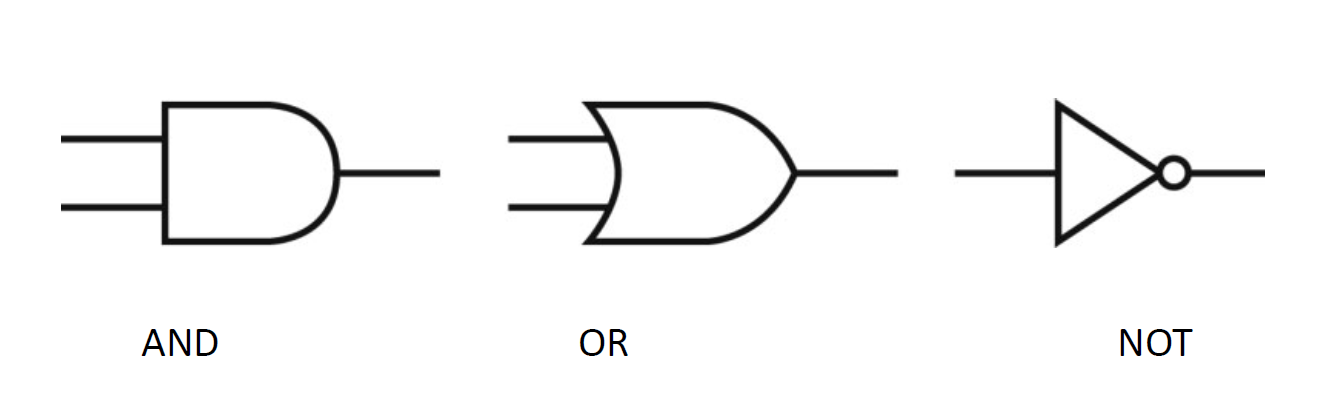
\includegraphics[width=0.8\textwidth,keepaspectratio]{images/porte_logiche.png}
	\caption{Rappresentazione di AND, OR e NOT}
\end{figure}

Si ricorda inoltre che è possibile combinare fra loro diverse porte logiche:
\begin{figure}[H]
	\centering
	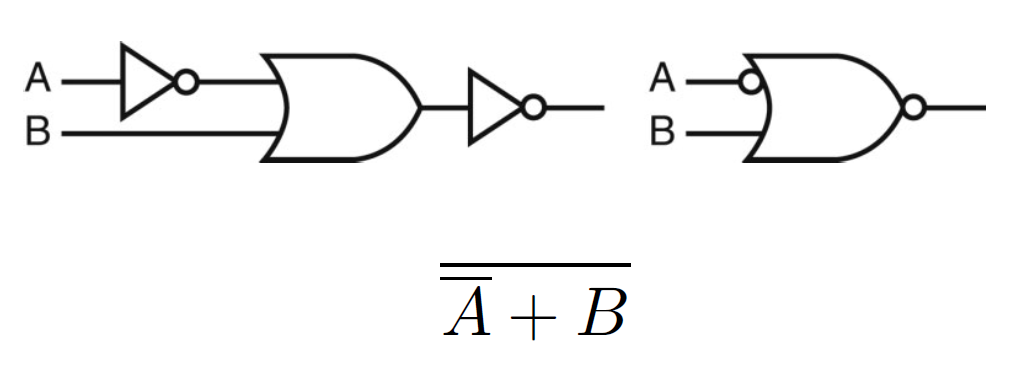
\includegraphics[width=0.8\textwidth,keepaspectratio]{images/combinazione_porte.png}
	\caption{Combinazione di porte logiche}
\end{figure}

\section{Alcuni circuiti degni di nota}
\subsection{Decoder}
L'ingresso del \emph{decoder} svolge il ruolo di selettore: ricevendo in input il valore \(n\), si accenderà l'\(n\)-esima uscita. A seguire l'implementazione di un decoder a 3 bit:
\begin{figure}[H]
	\centering
	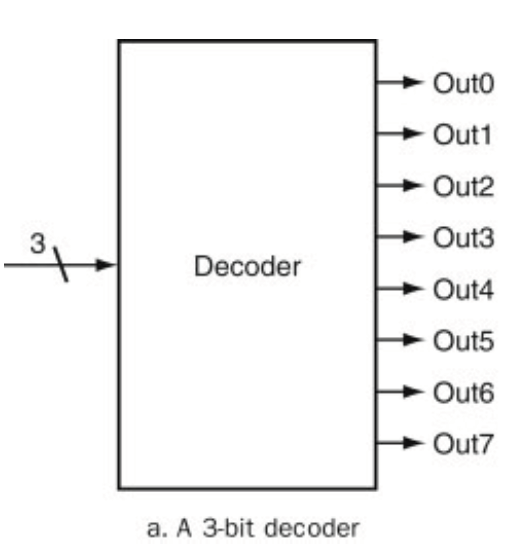
\includegraphics[width=0.4\textwidth,keepaspectratio]{images/3bit_decoder.png}
	\caption{Decoder a 3 bit}
\end{figure}
\begin{table}[!h]
	\centering
	\begin{tabular}{|c|c|c|c|c|c|c|c|c|c|c|}
		\hline
		\rowcolor[HTML]{EFEFEF} 
		\multicolumn{3}{|c|}{\cellcolor[HTML]{EFEFEF}Input} & \multicolumn{8}{c|}{\cellcolor[HTML]{EFEFEF}Output} \\ \hline
		\rowcolor[HTML]{EFEFEF} 
		In2 & In1 & In0 & Out7 & Out6 & Out5 & Out4 & Out3 & Out2 & Out1 & Out0 \\ \hline
		0 & 0 & 0 & 0 & 0 & 0 & 0 & 0 & 0 & 0 & 1 \\ \hline
		0 & 0 & 1 & 0 & 0 & 0 & 0 & 0 & 0 & 1 & 0 \\ \hline
		0 & 1 & 0 & 0 & 0 & 0 & 0 & 0 & 1 & 0 & 0 \\ \hline
		0 & 1 & 1 & 0 & 0 & 0 & 0 & 1 & 0 & 0 & 0 \\ \hline
		1 & 0 & 0 & 0 & 0 & 0 & 1 & 0 & 0 & 0 & 0 \\ \hline
		1 & 0 & 1 & 0 & 0 & 1 & 0 & 0 & 0 & 0 & 0 \\ \hline
		1 & 1 & 0 & 0 & 1 & 0 & 0 & 0 & 0 & 0 & 0 \\ \hline
		1 & 1 & 1 & 1 & 0 & 0 & 0 & 0 & 0 & 0 & 0 \\ \hline
	\end{tabular}
	\caption{Tabella di verità per un decoder a 3 bit}
	\label{decoder-3bit}
\end{table}

\subsection{Multiplexer}
Prevede un input con valore \(S\) utilizzato come selettore. L'output del \emph{multiplexer} è il valore dell'input \(S\)-esimo.
\begin{figure}[H]
	\centering
	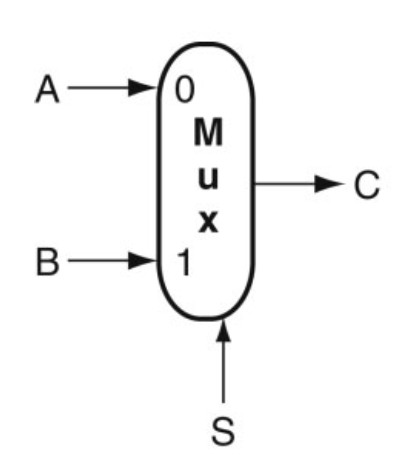
\includegraphics[width=0.3\textwidth,keepaspectratio]{images/multi.png}
	\caption{Multiplexer a 1 bit}
\end{figure}
\`{E} possibile costruire un multiplexer attraverso un decoder:
\begin{figure}[H]
	\centering
	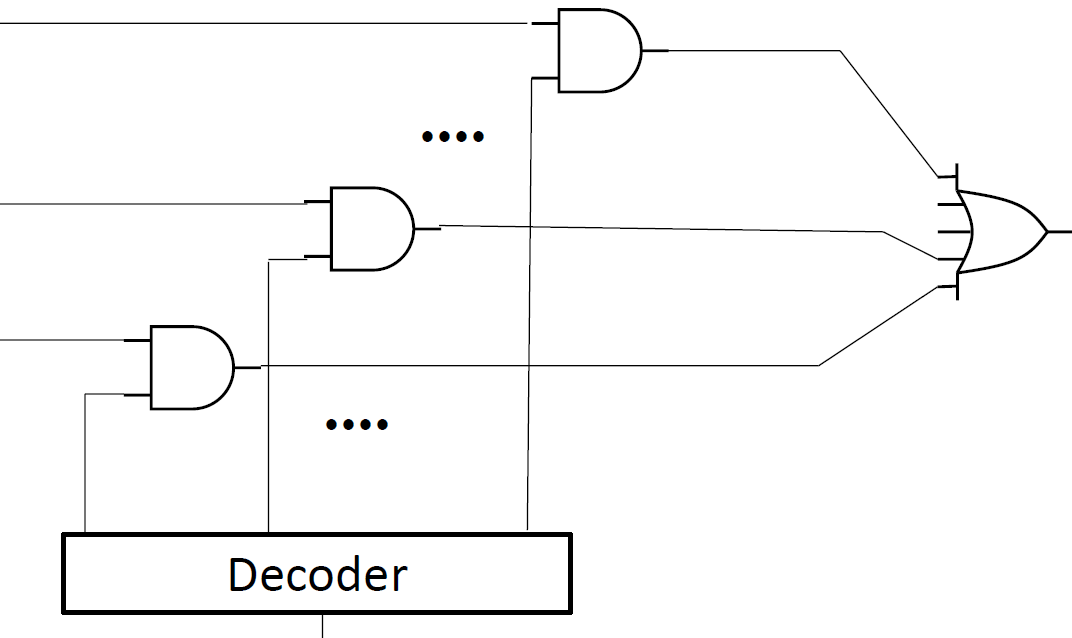
\includegraphics[width=0.7\textwidth,keepaspectratio]{images/multi_n_vie.png}
	\caption{Multiplexer a n vie}
\end{figure}
Molto spesso, per operare con dati complessi, si compongono degli array di elementi elementari. Segue un esempio di come sia possibile costruire un multiplexer a 32 bit utilizzando un array di multiplexer a 1 bit.
\begin{figure}[H]
	\centering
	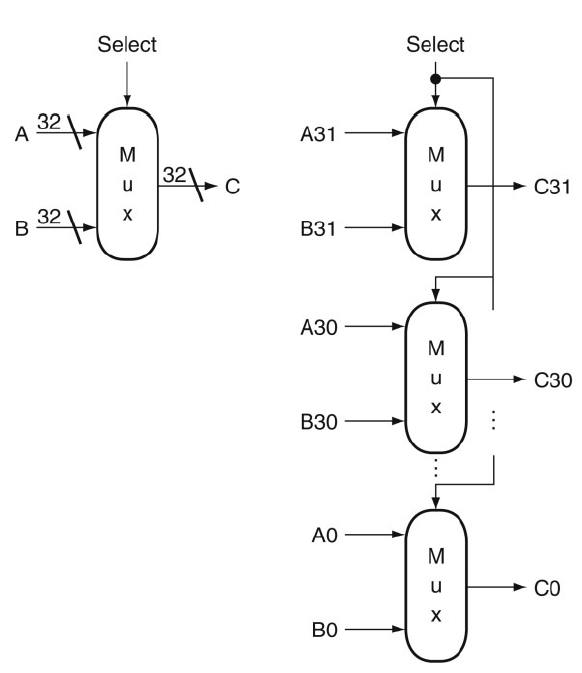
\includegraphics[width=0.7\textwidth,keepaspectratio]{images/mux_32bit.png}
	\caption{Multiplexer a 32 bit}
\end{figure}

\subsection{Programmable Logic Array (PLA)}
Il \emph{programmable logic array} si compone di due strutture: una barriera di AND e da una barriera di OR. La dimensione totale del \emph{PLA} è data dalla somma del piano AND (numero di mintermini) e del piano OR (numero di uscite).\\
Inoltre, il PLA implementa porte logiche solamente per le configurazioni che producono 1 in uscita. In aggiunta, se un mintermine è condiviso tra varie uscite, lo si può riutilizzare.
Successivamente seguono due diverse implementazioni della rete logica descritta nel paragrafo~\ref{subsec:mintermini}.
\begin{figure}[H]
	\centering
	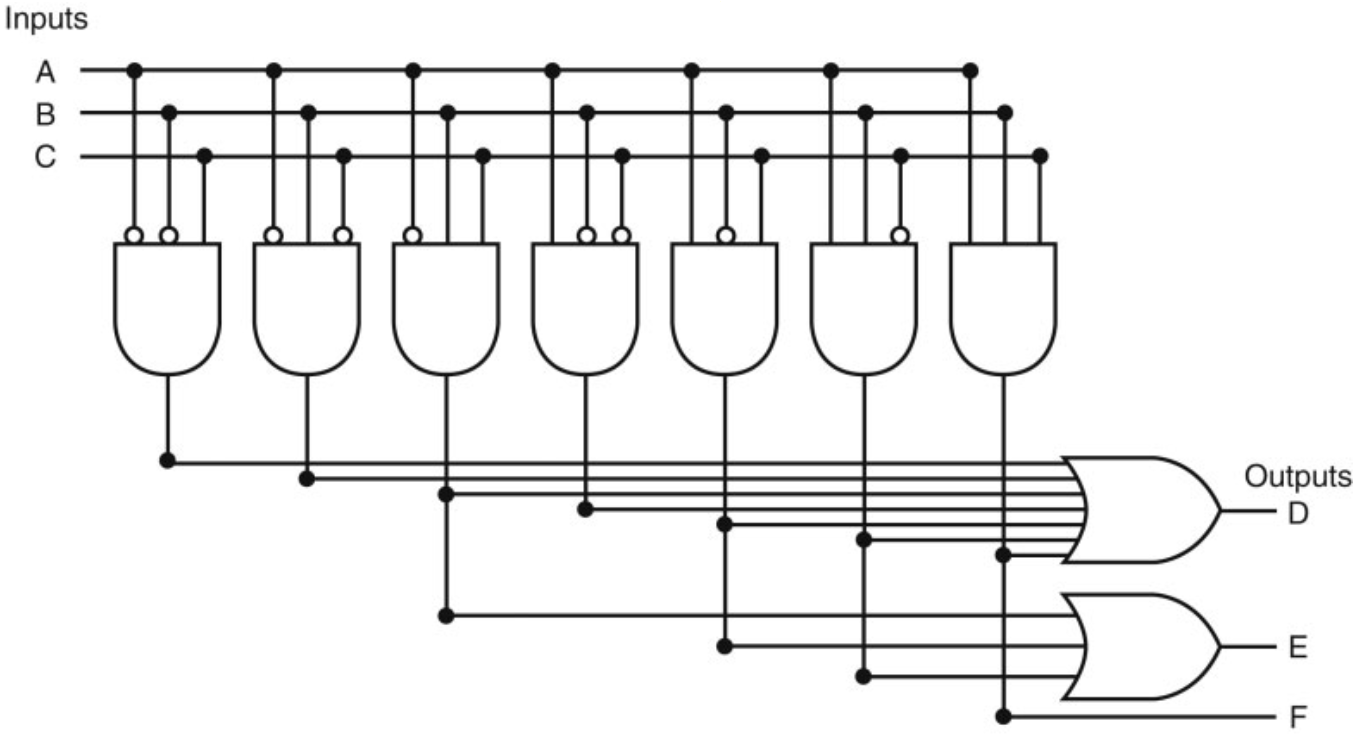
\includegraphics[width=0.7\textwidth,keepaspectratio]{images/es_rete_logica.png}
	\caption{Esempio di rete logica}
\end{figure}
\begin{figure}[H]
	\centering
	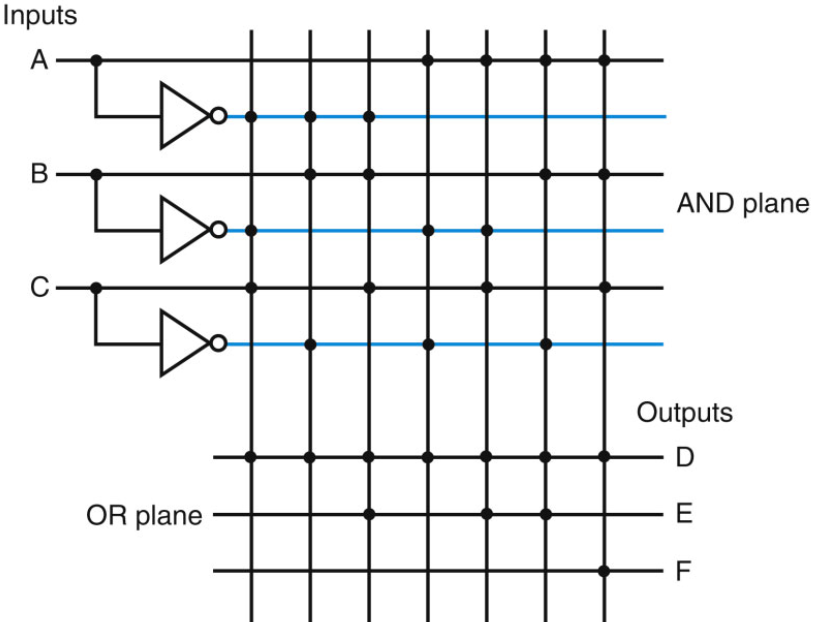
\includegraphics[width=0.7\textwidth,keepaspectratio]{images/es_pla.png}
	\caption{Esempio di rete logica implementata attraverso PLA}
\end{figure}

\section{Il concetto di \emph{costo}}
Come appena visto, le reti logiche possono essere implementate in maniera differente. Si definisce \emph{costo} di una rete logica la somma del numero di porte e del numero di ingressi della rete. Quando si analizza una rete, è importante saperne trovare l'implementazione con costo minimo. Principalmente si può procedere in due modalità:
\begin{itemize}[noitemsep]
	\item regole di semplificazione matematiche dovute all'algebra di Boole (vedi paragrafo~\ref{subsec:semplificazione}).
	\item metodi basati su rappresentazioni grafiche (mappe di \emph{Karnaugh}), nei casi più semplici.
\end{itemize}

\section{Le reti sequenziali}
Come si è visto, le reti combinatorie non hanno memoria degli stati del passato: in ogni istante di tempo l’uscita dipende solamente dagli ingressi nell’istante considerato. Tuttavia, in certe applicazioni è necessario introdurre una vera e propria memoria nel sistema.\\
La memoria in una rete logica si ottiene attraverso una \emph{retroazione}, che consiste nel ridirezionare alcune porte di uscita in ingresso ad altre porte del medesimo circuito, in maniera tale da formare un anello.\\
Seppur questo meccanismo offra delle potenzialità enormi, l'analisi e la sintesi di una rete logica è molto più complessa rispetto a quella delle reti combinatorie.

\subsection{Latch S-R}
A seguire un'implementazione di una rete sequenziale \emph{latch S-R} (\emph{set-reset}) costruita attraverso due porte NOR:
\begin{figure}[H]
	\centering
	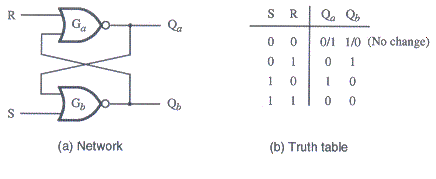
\includegraphics[width=0.8\textwidth,keepaspectratio]{images/es_latch.png}
	\caption{Esempio di latch a porte NOR}
\end{figure}
\begin{figure}[H]
	\centering
	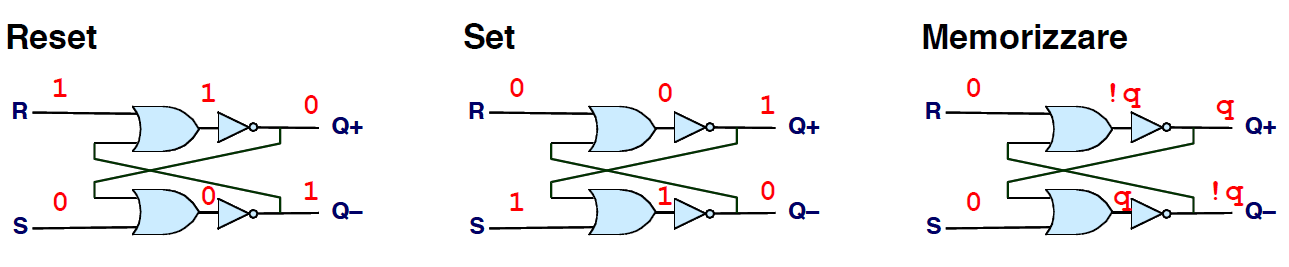
\includegraphics[width=\textwidth,keepaspectratio]{images/operazioni_latch.png}
	\caption{Operazioni di un latch a porte NOR}
\end{figure}
Ma, considerando che i segnali non si propagano in tempo nullo, ciò potrebbe causare dei problemi circa la correttezza del segnale stesso. La soluzione è quella di aggiungere un ulteriore segnale, in grado di temporizzare il circuito: il \emph{clock}. Un latch dotato di temporizzazione viene chiamato \emph{gated latch}.
\begin{figure}[H]
	\centering
	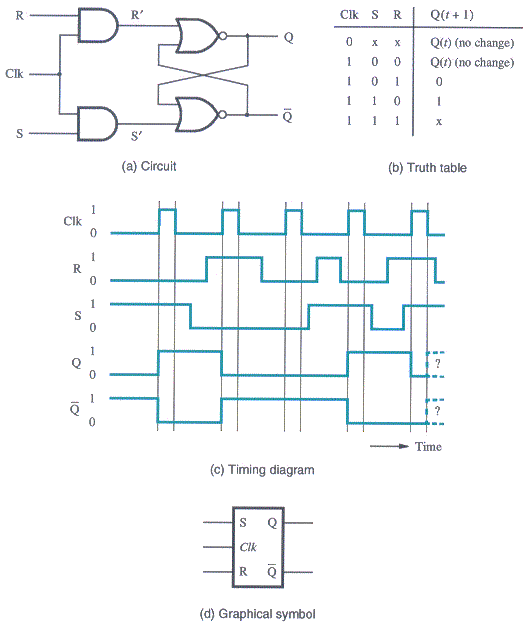
\includegraphics[width=\textwidth,keepaspectratio]{images/gated_latch.png}
	\caption{Esempio di gated latch}
\end{figure}
Il difetto principale di un latch R-S è quello di avere uno stato indecidibile: l'uscita non può essere nota con certezza quando entrambi gli ingressi sono a 1.

Una soluzione è implementata attraverso \emph{latch} tipo \emph{D}: gli ingressi al circuito sono ottenuti da un'unica variabile (di cui se ne fa il negato). Altrimenti, attraverso circuiti \emph{flip-flop master-slave} è possibile ottenere che l’uscita del circuito commuti esattamente al termine dell’impulso di clock. 




\backmatter
% bibliography, glossary and index would go here.

\end{document}